\section{Results}

\subsection{Sample and signal quality}
Of the 53 recordings, \NIncluded{} met the pre-specified quality criteria (\NIncludedMDD{} MDD, \NIncludedHC{} HC).
Exclusions affected \NExcludedMDD{} MDD and \NExcludedHC{} HC participants (Fisher's exact $p=\ExclusionFisherP$).
Among included participants, the median number of retained face-locked trials was \MedianTrials{} of 480
(range \MinTrials--\MaxTrials), the median number of interpolated channels was \MedianBadCh{} (range
\MinBadCh--\MaxBadCh) and the median number of removed ICA components was \MedianIca{} of 30 (range \MinIca--\MaxIca).
None of these quality measures differed between groups (Mann--Whitney $p=\QualNTrialsKeptTotalP$,
$\QualNBadChannelsP$ and $\QualIcaNExcludedP$, respectively; Fig.~\ref{fig:quality}). Any group difference in the
features is therefore unlikely to reflect a gross difference in data quality.

\subsection{Classification of MDD vs.\ HC}
Table~\ref{tab:main} and Fig.~\ref{fig:models} summarise all models. All estimates are participant-level and
out-of-sample.

\paragraph{Primary analysis.} The pre-specified primary model (LR-L2 on all 288 features) did not separate the
groups: AUC $=\PrimaryLrLAllAuc$ (95\% CI \PrimaryLrLAllAucLo--\PrimaryLrLAllAucHi), balanced accuracy
$=\PrimaryLrLAllBalancedAccuracy$, permutation $p=\PrimaryLrLAllPperm$ (Fig.~\ref{fig:perm}). The primary hypothesis,
that task EEG features classify MDD above chance in unseen participants, is therefore not supported.

\paragraph{Demographic baseline.} Age, sex and education alone gave AUC $=\DemographicsLrAuc$
(\DemographicsLrAucLo--\DemographicsLrAucHi, $p=\DemographicsLrPperm$). Of the three variables, only education differed between groups
(Table~\ref{tab:demo}), so it presumably carries most of this signal. This baseline outperformed the primary EEG model on the same folds (mean per-fold
$\Delta$AUC $=\CmpPrimaryLrLAllVsDemoDiff$, corrected resampled $t$-test $p=\CmpPrimaryLrLAllVsDemoP$;
Table~\ref{tab:cmp}). It was not exceeded by any EEG model.

\paragraph{Secondary models.} Of the secondary models, only L1-regularised logistic regression reached nominal
significance: AUC $=\LrLAllAuc$ (\LrLAllAucLo--\LrLAllAucHi), uncorrected permutation $p=\LrLAllPperm$. This result
does not survive Holm correction over the \NSecondaryHolm{} secondary models with permutation tests
($p_\text{Holm}=\LrLAllPholm$). Its advantage over the primary model on the same folds was also not significant
($\Delta$AUC $=\CmpLrLAllVsPrimaryDiff$, $p=\CmpLrLAllVsPrimaryP$).

The nested model-selection estimate is the honest estimate of ``choosing the best handcrafted-feature model'',
because the choice of model family is made inside the inner loop. It was lower: AUC $=\NestedmodelselectionAllAuc$
(\NestedmodelselectionAllAucLo--\NestedmodelselectionAllAucHi, $p=\NestedmodelselectionAllPperm$).

No single feature family was informative on its own. LR-L2 AUCs were:
\begin{itemize}
  \item spectral and FAA: \LrLSpectralAuc;
  \item ERP: \LrLErpAuc;
  \item connectivity: \LrLConnectivityAuc;
  \item complexity: \LrLComplexityAuc.
\end{itemize}
All permutation $p$-values were $\geq\LrLSpectralPperm$. Non-linear models (RBF SVM, random forest, LightGBM) did
not improve on linear ones.

\paragraph{Trial-level models.} Neither the Riemannian nor the deep-learning models exploited the trial-level data
better than the handcrafted features (Table~\ref{tab:main}).
\begin{itemize}
  \item Riemannian: tangent space + LR, AUC $=\TsLrAuc$; MDM, \MdmAuc; ERP covariances, \ErpcovTsLrAuc{}
        ($p=\ErpcovTsLrPperm$).
  \item Deep learning: EEGNet, AUC $=\DlEegnetAuc$; ShallowFBCSPNet, \DlShallowfbcspnetAuc; TCN, \DlTcnAuc.
        All confidence intervals include 0.5.
\end{itemize}
The deep networks reached high validation AUCs in some folds, but test AUCs fluctuated widely across folds. This is
the signature of fitting participant-specific rather than diagnosis-specific structure with only 36 training
participants per fold.

\begin{table}[t]
\centering\scriptsize
\setlength{\tabcolsep}{3.5pt}
\caption{Participant-level out-of-sample performance (MDD vs.\ HC, $n=\NIncluded$). Point estimates are means over
10 repetitions of 5-fold cross-validation (3 for deep learning). 95\% CIs come from a participant bootstrap.
Sensitivity and specificity are at a fixed 0.5 threshold. $p_\text{perm}$: label-permutation test re-running the
full nested pipeline (number of permutations in parentheses); ``--'' means not run. The primary model is in bold.}
\label{tab:main}
\begin{tabular}{@{}llllllr@{}}
\toprule
Model & AUC [95\% CI] & Bal.\ acc.\ [95\% CI] & Sens. & Spec. & Brier & $p_\text{perm}$ \\
\midrule
\multicolumn{7}{@{}l}{\textit{Demographic baseline}} \\
\quad Age + sex + education (LR) & 0.78 [0.63, 0.91] & 0.76 [0.63, 0.88] & 0.72 & 0.80 & 0.205 & 0.002 (1000) \\
\multicolumn{7}{@{}l}{\textit{Handcrafted features}} \\
\quad LR-L1, all features & 0.72 [0.56, 0.87] & 0.66 [0.51, 0.79] & 0.67 & 0.64 & 0.223 & 0.013 (1000) \\
\quad Nested model selection, all features & 0.63 [0.46, 0.79] & 0.60 [0.46, 0.74] & 0.62 & 0.57 & 0.253 & 0.080 (200) \\
\quad Random forest, all features & 0.55 [0.38, 0.72] & 0.55 [0.40, 0.70] & 0.52 & 0.59 & 0.253 & 0.348 (200) \\
\quad LightGBM, all features & 0.55 [0.37, 0.72] & 0.55 [0.41, 0.69] & 0.40 & 0.70 & 0.325 & 0.353 (200) \\
\quad \textbf{LR-L2, all features (primary)} & 0.53 [0.36, 0.70] & 0.54 [0.39, 0.69] & 0.46 & 0.62 & 0.259 & 0.456 (1000) \\
\quad Linear SVM, all features & 0.51 [0.34, 0.68] & 0.55 [0.40, 0.69] & 0.65 & 0.45 & 0.246 & 0.479 (1000) \\
\quad RBF SVM, all features & 0.43 [0.27, 0.61] & 0.50 [0.39, 0.62] & 0.76 & 0.25 & 0.269 & 0.572 (200) \\
\multicolumn{7}{@{}l}{\textit{Feature families}} \\
\quad LR-L2, complexity & 0.55 [0.38, 0.72] & 0.57 [0.43, 0.72] & 0.58 & 0.57 & 0.288 & 0.705 (1000) \\
\quad LR-L2, spectral + FAA & 0.51 [0.34, 0.68] & 0.54 [0.40, 0.69] & 0.48 & 0.60 & 0.282 & 0.325 (1000) \\
\quad LR-L2, wPLI connectivity & 0.47 [0.30, 0.65] & 0.46 [0.32, 0.61] & 0.39 & 0.54 & 0.304 & 0.768 (1000) \\
\quad LR-L2, ERP & 0.42 [0.25, 0.59] & 0.43 [0.28, 0.57] & 0.36 & 0.50 & 0.319 & 0.720 (1000) \\
\multicolumn{7}{@{}l}{\textit{Riemannian (trial level)}} \\
\quad ERP covariances + TS + LR & 0.61 [0.43, 0.78] & 0.56 [0.42, 0.70] & 0.44 & 0.67 & 0.246 & 0.159 (200) \\
\quad Tangent space + LR & 0.50 [0.32, 0.67] & 0.47 [0.32, 0.61] & 0.39 & 0.54 & 0.278 & 0.532 (200) \\
\quad MDM & 0.35 [0.20, 0.52] & 0.39 [0.25, 0.53] & 0.28 & 0.50 & 0.290 & 0.891 (200) \\
\multicolumn{7}{@{}l}{\textit{Deep learning (trial level)}} \\
\quad TCN & 0.48 [0.30, 0.65] & 0.48 [0.34, 0.63] & 0.41 & 0.56 & 0.287 & -- \\
\quad EEGNet & 0.47 [0.30, 0.65] & 0.46 [0.35, 0.58] & 0.17 & 0.75 & 0.324 & -- \\
\quad ShallowFBCSPNet & 0.44 [0.27, 0.61] & 0.48 [0.35, 0.62] & 0.31 & 0.65 & 0.350 & -- \\
\bottomrule
\end{tabular}
\end{table}

\begin{figure}[t]
\centering
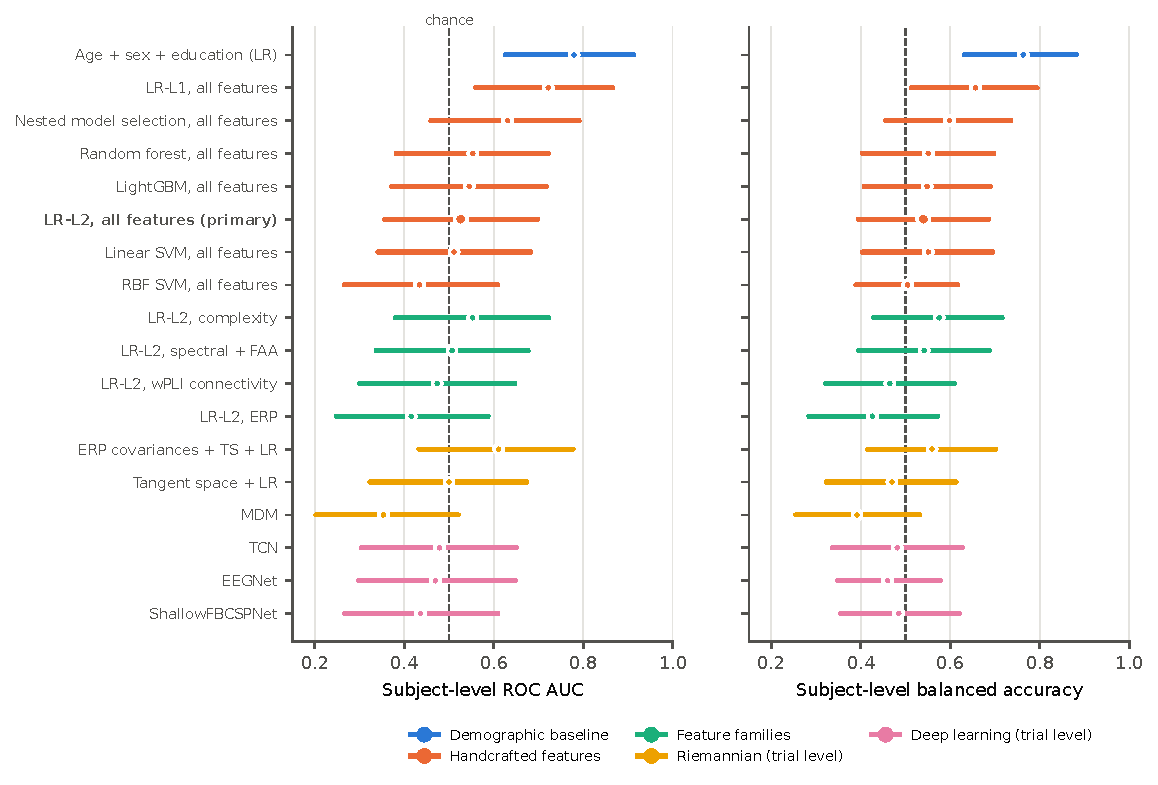
\includegraphics[width=\linewidth]{fig_model_comparison}
\caption{Participant-level ROC AUC (left) and balanced accuracy (right) with 95\% bootstrap CIs, for every model.
The dashed line marks chance. Only the demographic baseline (blue), which uses no EEG, has a CI clearly above
chance.}
\label{fig:models}
\end{figure}

\begin{table}[t]
\centering\scriptsize
\caption{Paired comparisons on identical participant folds. $\Delta$AUC is the mean per-fold difference
(model $-$ reference). $p_\text{corr}$ is from the corrected resampled $t$-test~\cite{nadeau2003inference}.
$p_\text{Holm}$ applies Holm's correction to the permutation $p$-values of the secondary models.}
\label{tab:cmp}
\begin{tabular}{@{}lrrrrrr@{}}
\toprule
 & \multicolumn{2}{c}{vs.\ primary} & \multicolumn{2}{c}{vs.\ demographics} & & \\
\cmidrule(lr){2-3}\cmidrule(lr){4-5}
Model & $\Delta$AUC & $p_\text{corr}$ & $\Delta$AUC & $p_\text{corr}$ & $p_\text{perm}$ & $p_\text{Holm}$ \\
\midrule
LR-L1, all features & +0.16 & 0.106 & -0.09 & 0.470 & 0.013 & 0.169 \\
Nested model selection, all features & +0.08 & 0.392 & -0.17 & 0.176 & 0.080 & 0.955 \\
Random forest, all features & +0.02 & 0.672 & -0.22 & 0.029 & 0.348 & 1.000 \\
LightGBM, all features & +0.01 & 0.944 & -0.24 & 0.020 & 0.353 & 1.000 \\
LR-L2, all features (primary) & -- & -- & -0.25 & 0.019 & 0.456 & -- \\
Linear SVM, all features & -0.13 & 0.422 & -0.38 & 0.004 & 0.479 & 1.000 \\
RBF SVM, all features & -0.13 & 0.429 & -0.38 & 0.008 & 0.572 & 1.000 \\
LR-L2, complexity & +0.06 & 0.517 & -0.19 & 0.107 & 0.705 & 1.000 \\
LR-L2, spectral + FAA & -0.01 & 0.903 & -0.26 & 0.011 & 0.325 & 1.000 \\
LR-L2, wPLI connectivity & -0.10 & 0.325 & -0.34 & 0.008 & 0.768 & 1.000 \\
LR-L2, ERP & -0.15 & 0.121 & -0.40 & 0.000 & 0.720 & 1.000 \\
ERP covariances + TS + LR & +0.08 & 0.455 & -0.17 & 0.164 & 0.159 & 1.000 \\
Tangent space + LR & -0.05 & 0.670 & -0.30 & 0.027 & 0.532 & 1.000 \\
MDM & -0.19 & 0.094 & -0.44 & 0.000 & 0.891 & 1.000 \\
TCN & -0.07 & 0.656 & -0.31 & 0.078 & -- & -- \\
EEGNet & -0.09 & 0.512 & -0.33 & 0.022 & -- & -- \\
ShallowFBCSPNet & -0.12 & 0.434 & -0.36 & 0.025 & -- & -- \\
\bottomrule
\end{tabular}
\end{table}

\begin{figure}[t]
\centering
\begin{subfigure}[t]{0.36\linewidth}
  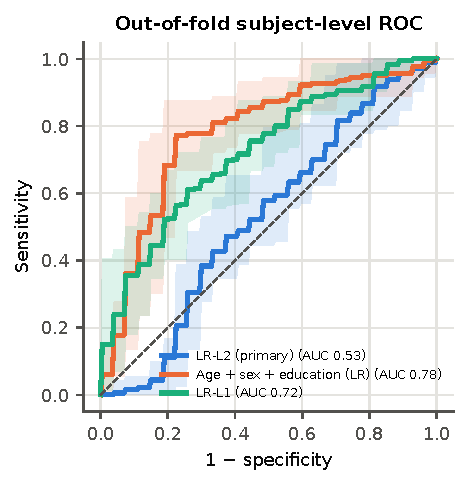
\includegraphics[width=\linewidth]{fig_roc}
  \caption{}
\end{subfigure}\hfill
\begin{subfigure}[t]{0.62\linewidth}
  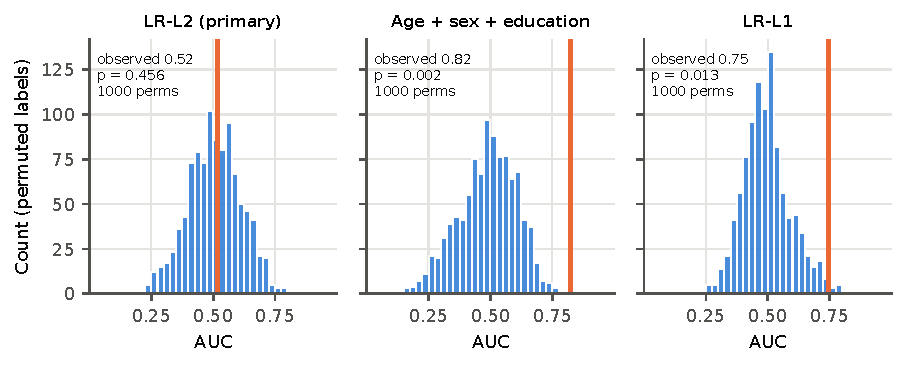
\includegraphics[width=\linewidth]{fig_permutation}
  \caption{}
\end{subfigure}
\caption{(a) Mean out-of-fold ROC curves across repetitions (band: 2.5--97.5\% range over repetitions).
(b) Permutation null distributions of the participant-level AUC, with the observed AUC (first repetition) marked.}
\label{fig:perm}
\end{figure}

\subsection{How much does trial-wise splitting inflate performance?}\label{sec:inflation}
Fig.~\ref{fig:inflation} contrasts the same two trial-level models under a trial-wise split, where trials of a
participant can fall in both training and test sets, and a subject-wise split.
\begin{itemize}
  \item \textbf{Tangent-space model.} Trial-level AUC was \InflTsLrTrialSplitTrialAuc{} with the trial-wise split and
        \InflTsLrSubjectSplitTrialAuc{} with the subject-wise split. Averaging trial probabilities per participant
        gave a participant-level AUC of \InflTsLrTrialSplitSubjectAuc{} under the trial-wise split, i.e.\ perfect
        apparent diagnosis, versus \InflTsLrSubjectSplitSubjectAuc{} under the subject-wise split.
  \item \textbf{Random forest on raw regional amplitudes}, the approach of many published studies and of an earlier
        unpublished analysis of these data by the author. Trial-level AUC was
        \InflRawamplitudeRfTrialSplitTrialAuc{} versus \InflRawamplitudeRfSubjectSplitTrialAuc, and participant-level
        AUC was \InflRawamplitudeRfTrialSplitSubjectAuc{} versus \InflRawamplitudeRfSubjectSplitSubjectAuc.
\end{itemize}
The trial-wise figures do not measure diagnosis. A classifier can recognise the \emph{participant} from the
individual statistics of their EEG, and the participant determines the label. Only the subject-wise figures answer
the clinical question.

The subject-wise participant-level AUC of the raw-amplitude random forest (\InflRawamplitudeRfSubjectSplitSubjectAuc)
is the highest of any EEG model. We do not interpret it as evidence of a diagnostic signal, for three reasons:
\begin{itemize}
  \item the model was included as a control, not pre-specified as a diagnostic model;
  \item it was evaluated with only three repetitions, and its post-hoc permutation test was borderline and did not
        survive multiplicity correction ($p=\AudRawRfP$, Holm $p=\AudRawRfPholm$; Section~\ref{sec:audit});
  \item it is one of many analyses, and for reference, 5\% of permutation runs of the primary pipeline exceeded AUC
        \PrimaryLrLAllNullQ.
\end{itemize}
It does suggest that the raw ERP waveform may be worth testing as a pre-specified hypothesis in independent data.

\begin{figure}[t]
\centering
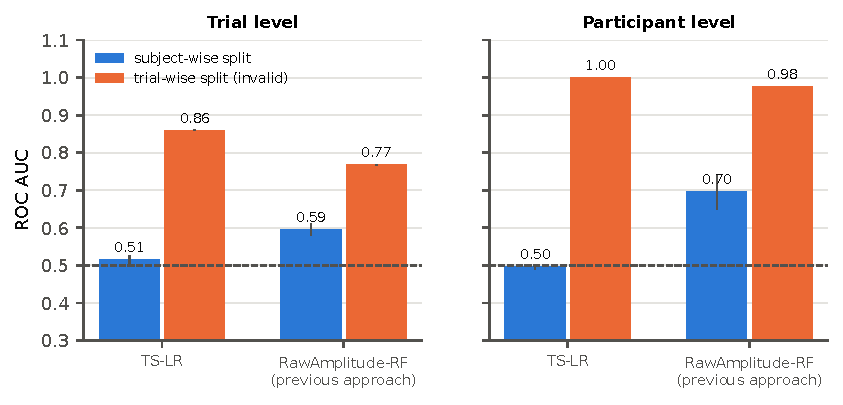
\includegraphics[width=0.85\linewidth]{fig_inflation}
\caption{AUC of the same models evaluated with a trial-wise split (invalid; trials of each participant appear in
training and test) and with a subject-wise split, at the trial level (left) and after averaging trial probabilities
per participant (right). Bars show means over three repetitions, with SD as error bars. The trial-wise split is shown
only to quantify the inflation.}
\label{fig:inflation}
\end{figure}

\subsection{Confounds and sensitivity analyses}
Table~\ref{tab:conf} reports whether the EEG features could predict variables other than diagnosis, using the
primary pipeline.
\begin{itemize}
  \item \textbf{Sex:} AUC $=\ConfSexAuc$ (\ConfSexAucLo--\ConfSexAucHi, $p=\ConfSexP$).
  \item \textbf{Age above the median:} \ConfAgeAuc{} ($p=\ConfAgeP$).
  \item \textbf{Recording period:} \ConfRecordingAuc{} ($p=\ConfRecordingP$).
\end{itemize}
EEG features thus carried information about sex, consistent with known sex differences in EEG amplitude and
spectra. Sex was balanced across groups (Table~\ref{tab:demo}), however, so it cannot explain a diagnostic signal,
and none was found. Neither age nor recording period was predictable from EEG.

Restricting the analysis to the \SensN{} participants recorded between June and August 2015 (\SensNMDD{} MDD), when
both groups were recorded in parallel, gave AUC $=\SensAuc$ (\SensAucLo--\SensAucHi, $p=\SensP$).

Including all 53 participants, with no exclusions, gave AUC $=\AllAuc$ (\AllAucLo--\AllAucHi, $p=\AllP$). The null
result is therefore not an artefact of the exclusion criteria. Primary-model AUC was similar in women
(\BySexFemaleAuc, $n=\BySexFemaleN$) and men (\BySexMaleAuc, $n=\BySexMaleN$).

\begin{table}[t]
\centering\small
\caption{Can the EEG features predict confounds? The primary pipeline (LR-L2, all features) was applied to
alternative targets, plus two sensitivity analyses of the MDD-vs-HC classification.}
\label{tab:conf}
\begin{tabular}{@{}lrll@{}}
\toprule
Target predicted from EEG features & $n_\text{pos}/n$ & AUC [95\% CI] & $p_\text{perm}$ \\
\midrule
sex (male) & 29/45 & 0.63 [0.45, 0.79] & 0.018 \\
age > median & 21/45 & 0.50 [0.33, 0.67] & 0.617 \\
recording period (>= Sep 2015) & 18/45 & 0.55 [0.37, 0.72] & 0.392 \\
\midrule
\multicolumn{4}{@{}l}{\textit{MDD vs.\ HC, primary pipeline, restricted subset}} \\
Recorded Jun--Aug 2015 & 9/25 & 0.46 [0.24, 0.70] & 0.517 \\
All 53 participants (no exclusions) & 24/53 & 0.57 [0.42, 0.72] & 0.278 \\
\bottomrule
\end{tabular}
\end{table}

\subsection{What, if anything, differs between groups?}
\paragraph{Model-based importance.} Permuting whole feature families in the test folds of the primary model
changed AUC by:
\begin{itemize}
  \item complexity: $\ImpComplexity$;
  \item spectral: $\ImpSpectral$;
  \item ERP: $\ImpErp$;
  \item connectivity: $\ImpConnectivity$.
\end{itemize}
All bootstrap intervals included zero (Fig.~\ref{fig:interp}a). SHAP values of the refitted primary model
(Fig.~\ref{fig:interp}b) were small in absolute terms, consistent with the strong regularisation selected.

\paragraph{Univariate effects.} \UniNSig{} of \UniNFeat{} features differed between groups at uncorrected $p<0.05$,
close to the $\approx14$ expected by chance. Only \UniNFdr{} survived false-discovery-rate correction: theta-band
wPLI between left central and left temporal regions ($d=\UniTopD$, $p_\text{FDR}=\UniTopPfdr$; Table~\ref{tab:uni}).

\paragraph{Spectral topography and ERPs.} Fig.~\ref{fig:topo} suggests higher beta and low-gamma power in MDD,
strongest at the edge of the montage, but no spatial cluster survived correction (minimum cluster
$p=\PowerClusterMinP$).

Group-average ERPs (Fig.~\ref{fig:erp}) showed the expected P1--N170 complex and a centro-parietal positivity in
both groups. Visually, MDD participants had a smaller late positivity at occipito-temporal sites, but the
spatio-temporal cluster test did not confirm any group difference (\ErpNClusters{} candidate clusters, minimum
$p=\ErpClusterMinP$).

\begin{figure}[t]
\centering
\begin{subfigure}[t]{0.40\linewidth}
  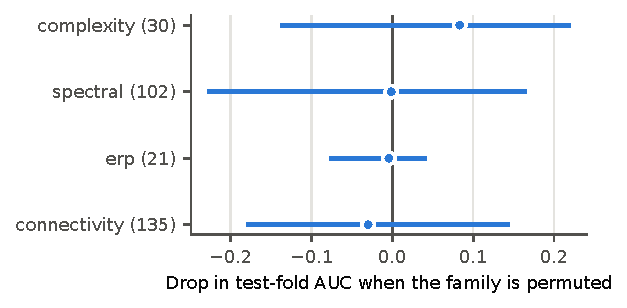
\includegraphics[width=\linewidth]{fig_family_importance}
  \caption{}
\end{subfigure}\hfill
\begin{subfigure}[t]{0.58\linewidth}
  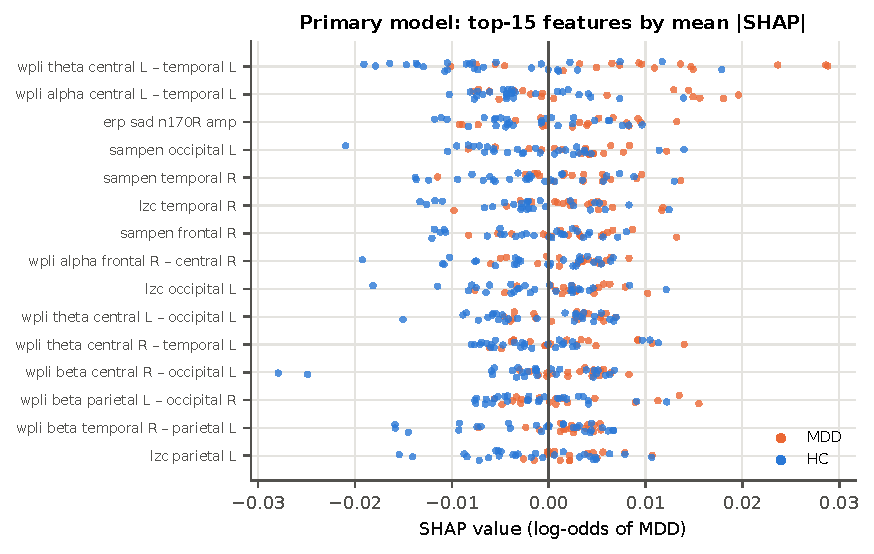
\includegraphics[width=\linewidth]{fig_shap}
  \caption{}
\end{subfigure}
\caption{(a) Drop in test-fold AUC of the primary model when each feature family is permuted jointly (mean and 95\%
interval over 50 outer folds; number of features in parentheses). (b) SHAP values of the primary model refitted on
all participants, for the 15 features with the largest mean $|$SHAP$|$ (descriptive).}
\label{fig:interp}
\end{figure}

\begin{figure}[t]
\centering
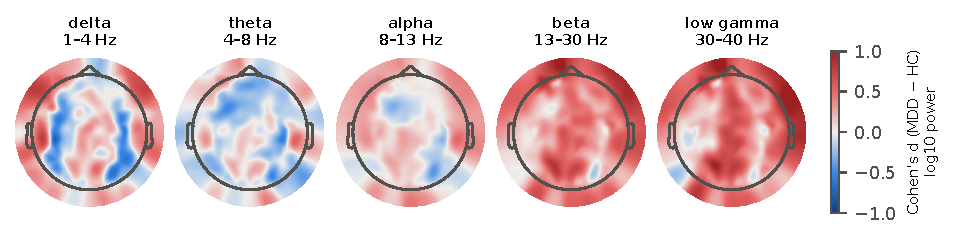
\includegraphics[width=\linewidth]{fig_topomaps_power}
\caption{Group differences in log band power per electrode (Cohen's $d$, MDD $-$ HC). Electrodes belonging to a
significant cluster (cluster permutation test, $p<0.05$) would be marked; none were.}
\label{fig:topo}
\end{figure}

\begin{figure}[t]
\centering
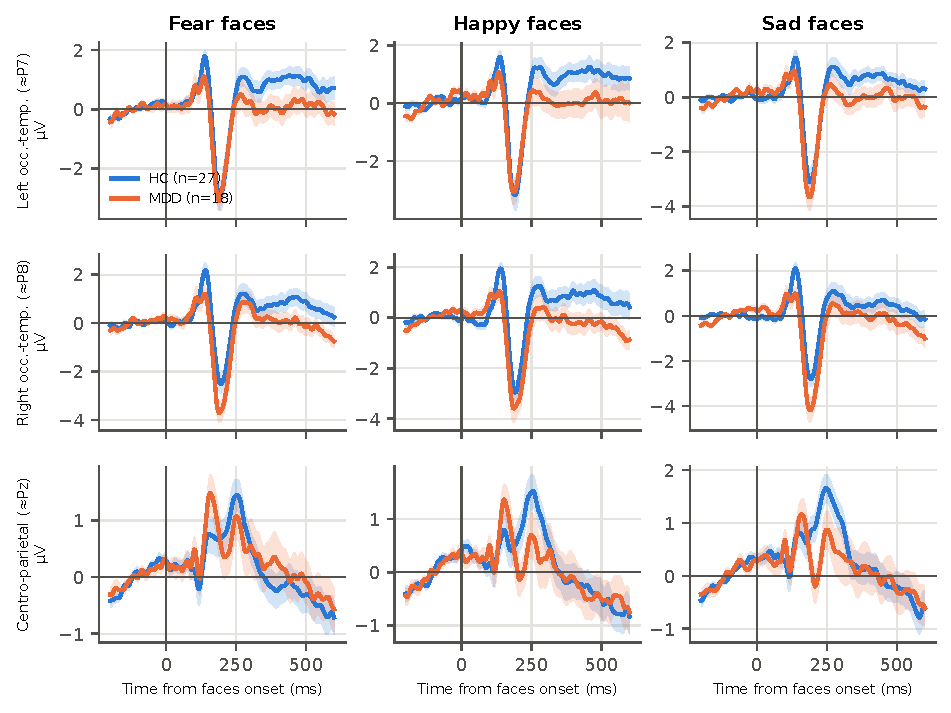
\includegraphics[width=\linewidth]{fig_erp_groups}
\caption{Grand-average ERPs ($\pm$SEM) per group and face condition, at the left and right occipito-temporal
clusters and the centro-parietal cluster. Shaded windows are the a-priori N170 (140--200~ms) and P300 (250--500~ms)
measurement windows.}
\label{fig:erp}
\end{figure}

\subsection{Post-hoc audit analyses (exploratory)}\label{sec:audit}
The analyses in this section were added after all pre-specified results were known (deviation D6;
Section~\ref{sec:audit-methods}). Table~\ref{tab:audit} lists the classification models. None of them changes the
conclusion.

\paragraph{Does EEG add to demographics?} No.
\begin{itemize}
  \item Adding all 288 EEG features to age, sex and education gave AUC $=\AudDemoPlusEEGAllAuc$
        (\AudDemoPlusEEGAllLo--\AudDemoPlusEEGAllHi). Permuting the EEG block gave $p=\AudDemoPlusEEGAllP$.
  \item Adding the compact set gave AUC $=\AudDemoPlusCompactAuc$ ($p=\AudDemoPlusCompactP$).
\end{itemize}
Both are \emph{below} the demographic baseline alone (\DemographicsLrAuc). With 45 participants, noisy EEG features
dilute rather than complement the demographic signal.

\paragraph{Is the null result an artefact of confounding or redundancy?} No.
\begin{itemize}
  \item EEG with age, sex and education regressed out inside each fold: AUC $=\AudEEGAlldeconfoundedAuc$
        ($p=\AudEEGAlldeconfoundedP$).
  \item PCA inside the fold: \AudEEGAllPCALRAuc{} ($p=\AudEEGAllPCALRP$).
  \item The compact theory-driven set, including the ERP contrasts between emotions, the aperiodic exponent, the
        alpha peak frequency and frontal-midline theta: \AudCompactLRAuc{} ($p=\AudCompactLRP$).
  \item Subject-level Riemannian model: \AudSubjectRiemannTSLRAuc{} ($p=\AudSubjectRiemannTSLRP$).
  \item Reaction times alone: \AudBehaviourRTLRAuc{} ($p=\AudBehaviourRTLRP$). Median RT was \AudRtMdd{} ms in MDD
        and \AudRtHc{} ms in HC ($p=\AudQRtIncP$).
\end{itemize}
The smallest uncorrected $p$ among these models was \AudMinP{}, and the smallest Holm-corrected $p$ was
\AudMinPholm.

\paragraph{Education as an EEG confound.} The EEG features did not predict education above the median: AUC
$=\AudEduAuc$ (\AudEduLo--\AudEduHi), $p=\AudEduP$. Only \AudEduNsig{} of 288 features correlated with education at
$p<0.05$, about the number expected by chance, and \AudEduNfdr{} survived FDR correction.

\paragraph{Residual muscle activity.} The EMG index, computed on the raw recordings, did not differ between groups
($p=\AudQEmgRelAllP$ in all 53 participants). It did, however, track the features that looked descriptively larger in
MDD (Fig.~\ref{fig:emg}):
\begin{itemize}
  \item mean sample entropy, $\rho=\AudEmgRSampen$;
  \item mean Lempel--Ziv complexity, $\rho=\AudEmgRLzc$;
  \item relative beta power, $\rho=\AudEmgRBeta$;
  \item relative 30--40~Hz power, $\rho=\AudEmgRGamma$;
  \item aperiodic exponent, $\rho=\AudEmgRApExp$ (all $p\le0.004$).
\end{itemize}
These families therefore index muscle tone as much as brain activity. The aperiodic exponent was nominally lower in
MDD ($p=\AudQApExpAllP$ in all 53; $p=\AudQApExpIncP$ in the 45 included). Given its correlation with the EMG index,
this cannot be attributed to cortical excitation--inhibition balance. The FDR-surviving wPLI feature was not related
to the EMG index ($\rho=\AudEmgRWpli$).

\paragraph{Signal quality before exclusion.} In all 53 participants, MDD and HC did not differ in:
\begin{itemize}
  \item retained trials ($p=\AudQTrialsAllP$);
  \item bad channels ($p=\AudQBadChAllP$);
  \item removed ICA components ($p=\AudQIcaAllP$) or ICLabel muscle components ($p=\AudQIcaMuscleAllP$).
\end{itemize}

\paragraph{Power.} The 95th percentile of the primary permutation null was AUC \AudPowThr. Even a perfect, already
trained score would exceed it with probability:
\begin{itemize}
  \item \AudPowIdealSeventy\% at true AUC 0.70;
  \item \AudPowIdealSeventyFive\% at 0.75;
  \item \AudPowIdealEighty\% at 0.80.
\end{itemize}
In the semi-synthetic analysis, where the primary pipeline has to learn the effect from 36 participants, power was
lower (Fig.~\ref{fig:power}a):
\begin{itemize}
  \item \AudSemiFivePower\% when the injected signal had an oracle AUC of \AudSemiFiveOracle;
  \item \AudSemiEightPower\% at oracle AUC \AudSemiEightOracle;
  \item \AudSemiTenPower\% at oracle AUC \AudSemiTenOracle.
\end{itemize}
The study could therefore only detect large effects. We extrapolated the same ideal score to larger samples, with
the same class ratio and one-sided $\alpha=0.05$. Reaching 80\% power would need about:
\begin{itemize}
  \item \AudNNeedSeventy{} participants for a true AUC of 0.70;
  \item \AudNNeedSixtyFive{} for 0.65;
  \item \AudNNeedSixty{} for 0.60.
\end{itemize}
These are optimistic lower bounds, because a pipeline that also has to learn the effect needs more.

\paragraph{Learning curve.} Between 12 and 36 training participants (Fig.~\ref{fig:power}b):
\begin{itemize}
  \item the primary model moved from AUC \AudLcPrimMin{} to \AudLcPrimMax;
  \item the demographic model moved from \AudLcDemoMin{} to \AudLcDemoMax.
\end{itemize}

\paragraph{Why trial-wise splits inflate.} A classifier on single-trial regional covariances identified \emph{which}
of the 45 participants produced a trial with \AudIdentAcc\% accuracy (chance \AudIdentChance\%). Individual EEG
signatures are thus highly distinctive, which explains the perfect participant-level AUC under trial-wise splitting
(Section~\ref{sec:inflation}).

\paragraph{Raw-amplitude random forest.} With the settings of its first repetition (AUC \AudRawRfObs), a permutation
test of the full subject-wise pipeline gave $p=\AudRawRfP$. The test used \AudRawRfN{} permutations, of which
\AudRawRfExceed{} reached the observed AUC, and the null 95th percentile was \AudRawRfQ. This is the only nominally
significant EEG result of the audit, but it is fragile:
\begin{itemize}
  \item with so few permutations, the 95\% interval for the exceedance probability extends to \AudRawRfPciHi;
  \item after Holm correction across the \AudRawRfFamily{} exploratory models it is $p=\AudRawRfPholm$;
  \item the model was not pre-specified, and a 288-feature linear model on summaries of the same data was at chance.
\end{itemize}
We therefore treat the raw ERP waveform as the most promising hypothesis this study generates, to be tested in
independent data, and not as a finding.

\begin{table}[t]
\centering\scriptsize
\setlength{\tabcolsep}{3pt}
\caption{Exploratory post-hoc models (D6), on the same folds as Table~\ref{tab:main}. $p_\text{perm}$: 1{,}000
permutations of the full nested pipeline. For the two incremental models the EEG block is permuted instead of the
labels. $p_\text{Holm}$ is computed across these seven models. $\Delta$AUC is the difference from the demographic
baseline, with the corrected resampled $t$-test.}
\label{tab:audit}
\begin{tabular}{@{}lccccc@{}}
\toprule
Model (exploratory, post hoc) & AUC [95\% CI] & BalAcc & $p_\text{perm}$ & $p_\text{Holm}$ & $\Delta$AUC vs demo ($p_\text{corr}$) \\
\midrule
Demographics + all 288 EEG features & 0.52 [0.35, 0.69] & 0.54 & 0.746 & 1.000 & -0.25 (0.014) \\
Demographics + compact EEG set & 0.59 [0.42, 0.75] & 0.59 & 0.584 & 1.000 & -0.17 (0.089) \\
EEG 288, age/sex/education regressed out in-fold & 0.49 [0.32, 0.66] & 0.50 & 0.703 & 1.000 & -0.28 (0.009) \\
EEG 288, PCA (in-fold) + LR & 0.58 [0.42, 0.75] & 0.58 & 0.381 & 1.000 & -0.18 (0.085) \\
Compact theory-driven EEG set (36) & 0.51 [0.34, 0.68] & 0.53 & 0.502 & 1.000 & -0.27 (0.009) \\
Reaction times only (8) & 0.44 [0.27, 0.62] & 0.49 & 0.726 & 1.000 & -0.37 (0.002) \\
Subject-mean covariance, tangent space + LR & 0.53 [0.35, 0.70] & 0.49 & 0.064 & 0.448 & -0.28 (0.065) \\
\bottomrule
\end{tabular}
\end{table}

\begin{figure}[t]
\centering
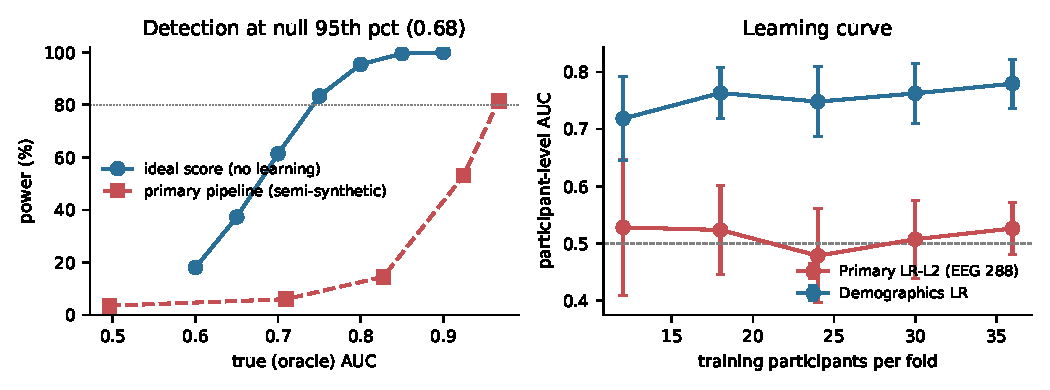
\includegraphics[width=\linewidth]{fig_power_curve}
\caption{(a) Probability of exceeding the 95th percentile of the permutation null, as a function of the true AUC. Blue:
an ideal pre-trained score. Red: the primary pipeline learning an injected effect, semi-synthetic. (b) Learning curve
(mean $\pm$ SD over 10 repetitions).}
\label{fig:power}
\end{figure}

\begin{figure}[t]
\centering
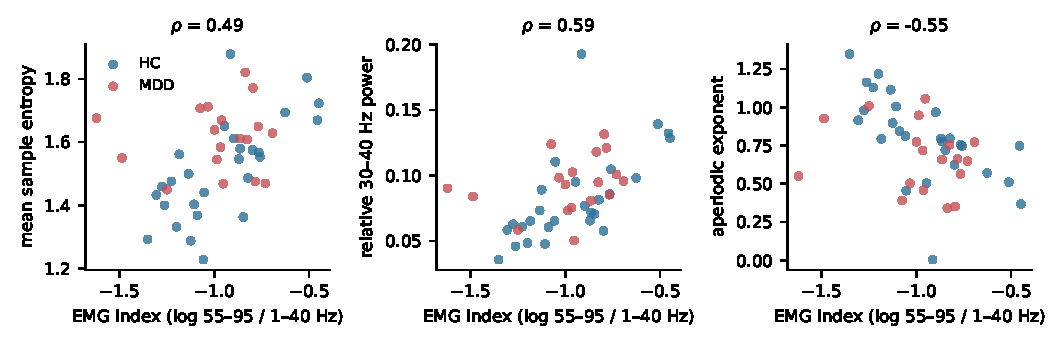
\includegraphics[width=\linewidth]{fig_emg}
\caption{EMG index (raw recordings) against global sample entropy, relative 30--40~Hz power and the aperiodic
exponent in the 45 included participants. $\rho$: Spearman correlation.}
\label{fig:emg}
\end{figure}
